\section{background}
\label{sec:background}

\subsection{Backlight scaling}
A visible image on LCD display is produced by both backlight and LCD
panel, which stores pixels color imformation. The perceptual luminance
is actually the backlight intensity compensated by the pixels. The
backlight scaling is a dedicated technique for LCD screen exploiting
this characteristics. This technique can be clearly illustrated in the
figure~\ref{fig:backlightscaling}. The energy of displaying one
picture can only be reduced by dimming the backlight, though it leads
to a darker version of this image. This distortion can be compensated
by concurrently increasing the luminance component of each pixel in
this image~\cite{PMLDV03, CHP07, CCS06, CSC02}. Fortunately, the
pixels brightness is uncorrelated to the power consumption of the
display.


\begin{figure}[!htb]
  \begin{center}
    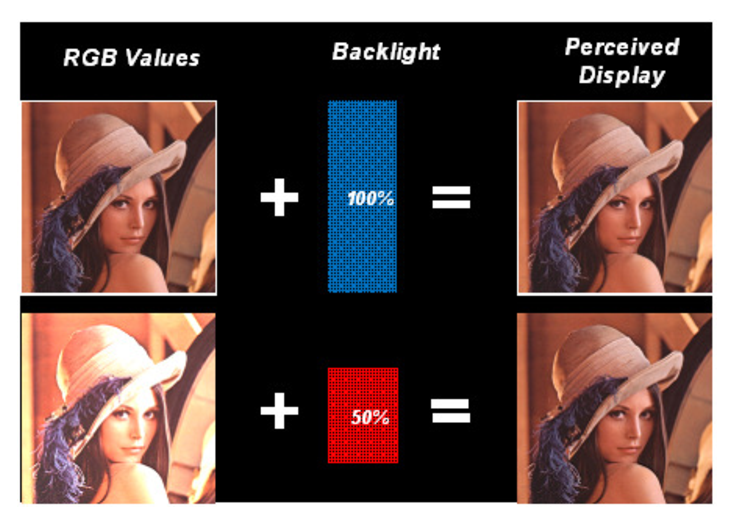
\includegraphics[scale=.75]{./figures/backlightscaling.eps}
    \caption{Backlight Scaling on LCD screen}
    \label{fig:backlightscaling}
  \end{center}
\end{figure}

Applying this technique in the video playbacks raises several
challenges. Both extracting and enhancing the pixels luminance
component frame by frame are the operations of processing a mass of
data. For this reason, deploying these tasks on the CPU~\cite{CHP07,
  CSC02} is not practical. On the one hand, the CPU may don't have
enough time to do these computation intensive tasks without degrading
the frames per second (FPS) of the video. On the other hand, the
achieved power savings by dimming backlight might be offset by these
extra operations. Hsiu et al. and Lin et al. ~\cite{LHH14, HLH11} proposed to
skip the pixels compensation stage and use a critical backlight level
of each frame to avoid distorting the image too badly. Ruggiero et
al. offload the luminance adjustment tasks to an independent
processor~\cite{RBB08}. Pasricha et al.~\cite{PMLDV03} and Cheng et
al.~\cite{CMEDV07} suggested to compute the backlight scaling data on
a proxy server and substitute the original video with a
luminance-adjusted version.


\subsection{WebRTC}

The conversational RTC protocols are the company proprietaries,
precluding the communication between different services.  The
prosperity of mobile devices, including the smartphones, the tablet
and emerging wearable devices, makes the situation more
complicated. To solve the fragmentation problem in the real-time
multimedia communication and also to provide a cross-platform
solution, Web Real-Time Communication (WebRTC)~\cite{webrtcstandard}
is proposed and standardized by the W3C and IETF. Nowadays, mainstream
browsers, e.g. Chrome, Firefox, Opera and etc., all have integrated
the WebRTC inside them. Not only does the WebRTC
component~\cite{webrtcproject} implemented in the Chrome provide the
Javascript-style APIs, but also it can be linked to the native mobile
apps as an external libary. In this paper, we build our prototype
based on the AppRTC, which is the Android version app incorperating
the WebRTC library.
